%!TeX encoding = UTF-8
%!TeX root = ../main.tex
\chapter{Dataset Management}
\label{chapter:dataset-management}

This section explains how to manage and organize datasets for our various customers.

\section{Introduction}

The general rules for dataset management are these:

\begin{itemize}
    \item Data is stored in Microsoft Azure
    \item Data is stored as Azure File Share during working phase
    \item Data is stored in Azure blobs when frozen
    \item Access rights must be set:
    \begin{itemize}
        \item Per developer for general dataset management
        \item Per project for technical dataset access
    \end{itemize}
\end{itemize}

\section{Dataset storage management}

Here's the general outline.

\begin{enumerate}
    \item Create a storage account (and possibly a resource group) on Microsoft Azure
    \item Create a Blob and a FileShare called "dataset"
    \item Generate a SAS key for your customer
    \item Download Azure Storage Explorer (see \url{https://azure.microsoft.com/en-us/features/storage-explorer/})
    \item Use Azure Storage Explorer to get the SAS link as explained here: \url{https://blogs.msdn.microsoft.com/jpsanders/2017/10/12/easily-create-a-sas-to-download-a-file-from-azure-storage-using-azure-storage-explorer/}
    \item Transmit this information to your customer using \url{dead-drop.me}.
\end{enumerate}

\subsection{Create storage account from Azure}

\begin{itemize}
    \item Connect to Azure portal
    \item Go to "Storage accounts"
    \item Create an account for your customer\footnote{Use full lowercase for customer name}
    \item Don't forget to create a resource group for your customer\footnote{Use same capitalization as your customer's real name}
\end{itemize}


%!TeX encoding = UTF-8
%!TeX root = ../main.tex
\chapter{Dataset Management (user manual)}
\label{chapter:customer-dataset-management}

This chapter explains how to access your dataset folders in order to push (or retrieve) your data in NumeriCube's platform.

\section{Prerequisites}

Download and install Azure Storage Explorer from the following URL: \url{https://azure.microsoft.com/en-us/features/storage-explorer/}.

Azure Storage Explorer is available for \texttt{Windows}, \texttt{Mac OS X} and \texttt{Linux}.

Make sure you received a \texttt{dead-drop.me} link with a password. Use this link to copy in your clipboard the Azure Shared Access Signature URI that you will use to authenticate on the file server.

\section{File share configuration}

\begin{itemize}
    \item Install Azure Storage Explorer
    \item Fetch the Azure Shared Access Signature URI from the link you received from \texttt{dead-drop.me}.
    \item Open the Azure Storage Explorer application
    \item Click on the electrical plug on the left (see \ref{figure:az-step1})
        \begin{figure}
        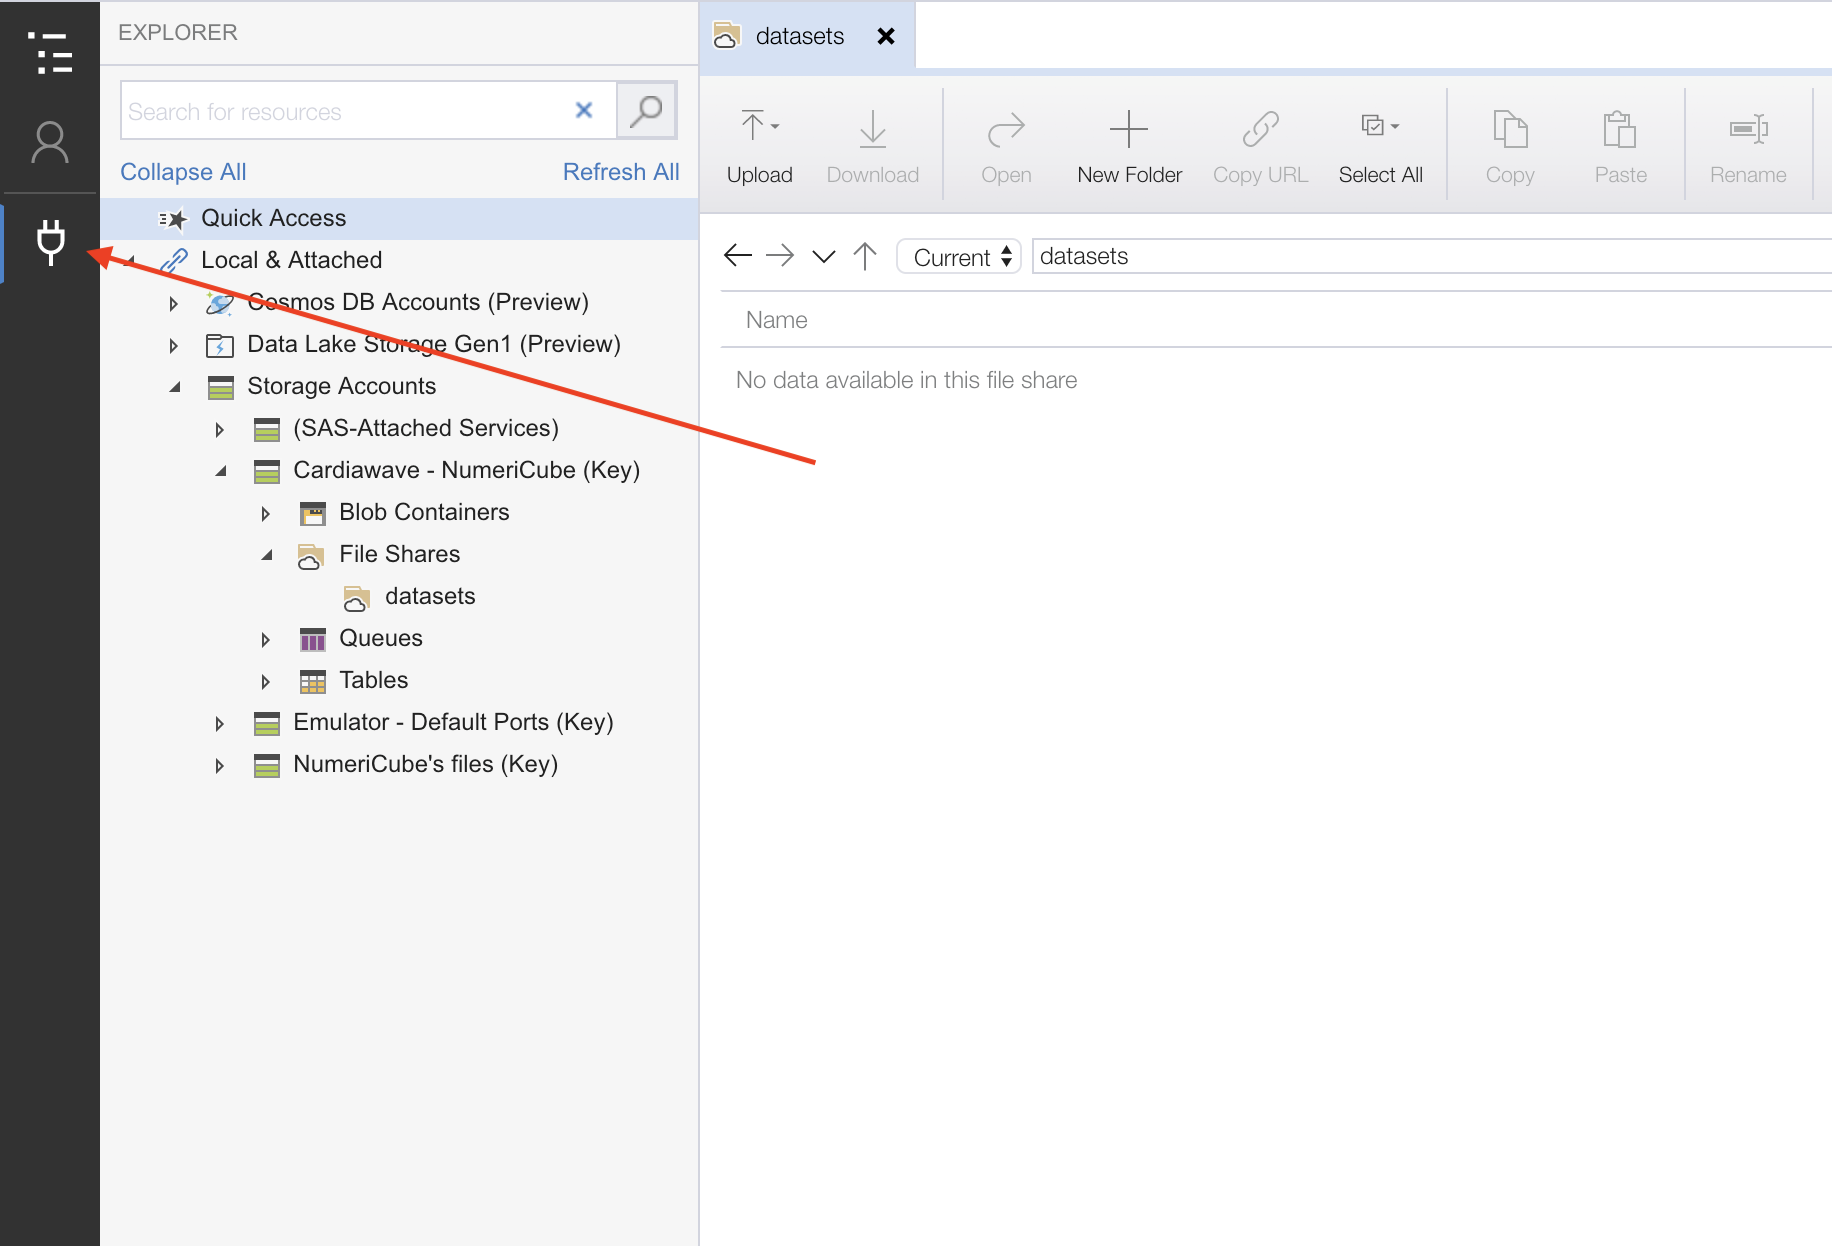
\includegraphics[width=\textwidth]{assets/az-step1.png}
        \caption{Connect to a new Azure file share}
        \label{figure:az-step1}
        \end{figure}
    \item Click the "Use Shared Access Signature URI" option and click \texttt{Next} (see \ref{figure:az-step2})
        \begin{figure}
        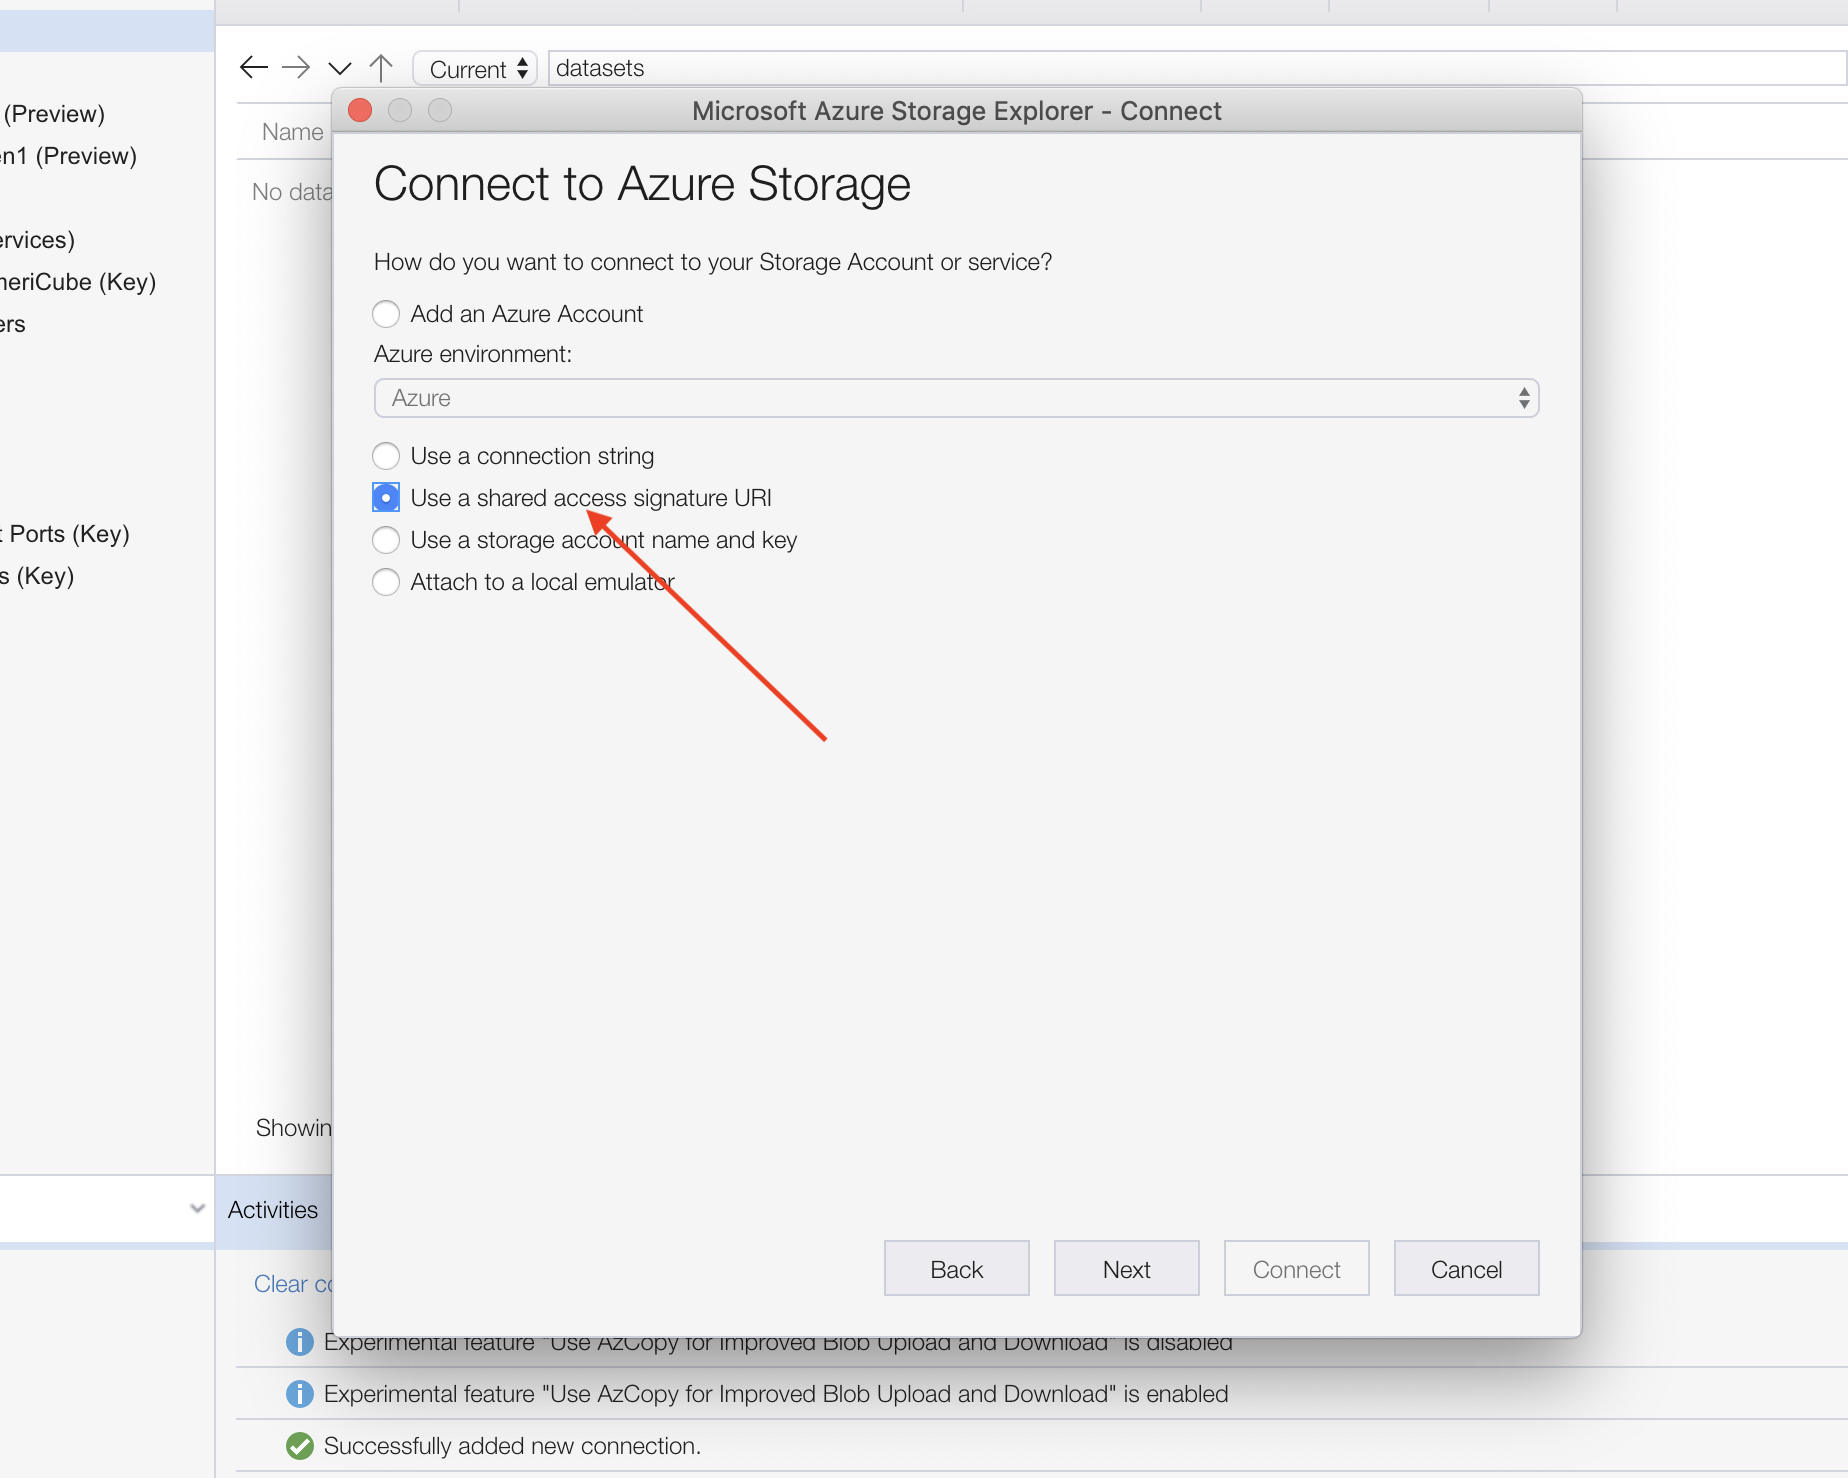
\includegraphics[width=\textwidth]{assets/az-step2.png}
        \caption{Connect to a new Azure file share}
        \label{figure:az-step2}
        \end{figure}
    \item Paste your Azure Shared Access Signature URI in the \texttt{URI} field and click \texttt{Next} (see \ref{figure:az-step3})
        \begin{figure}
        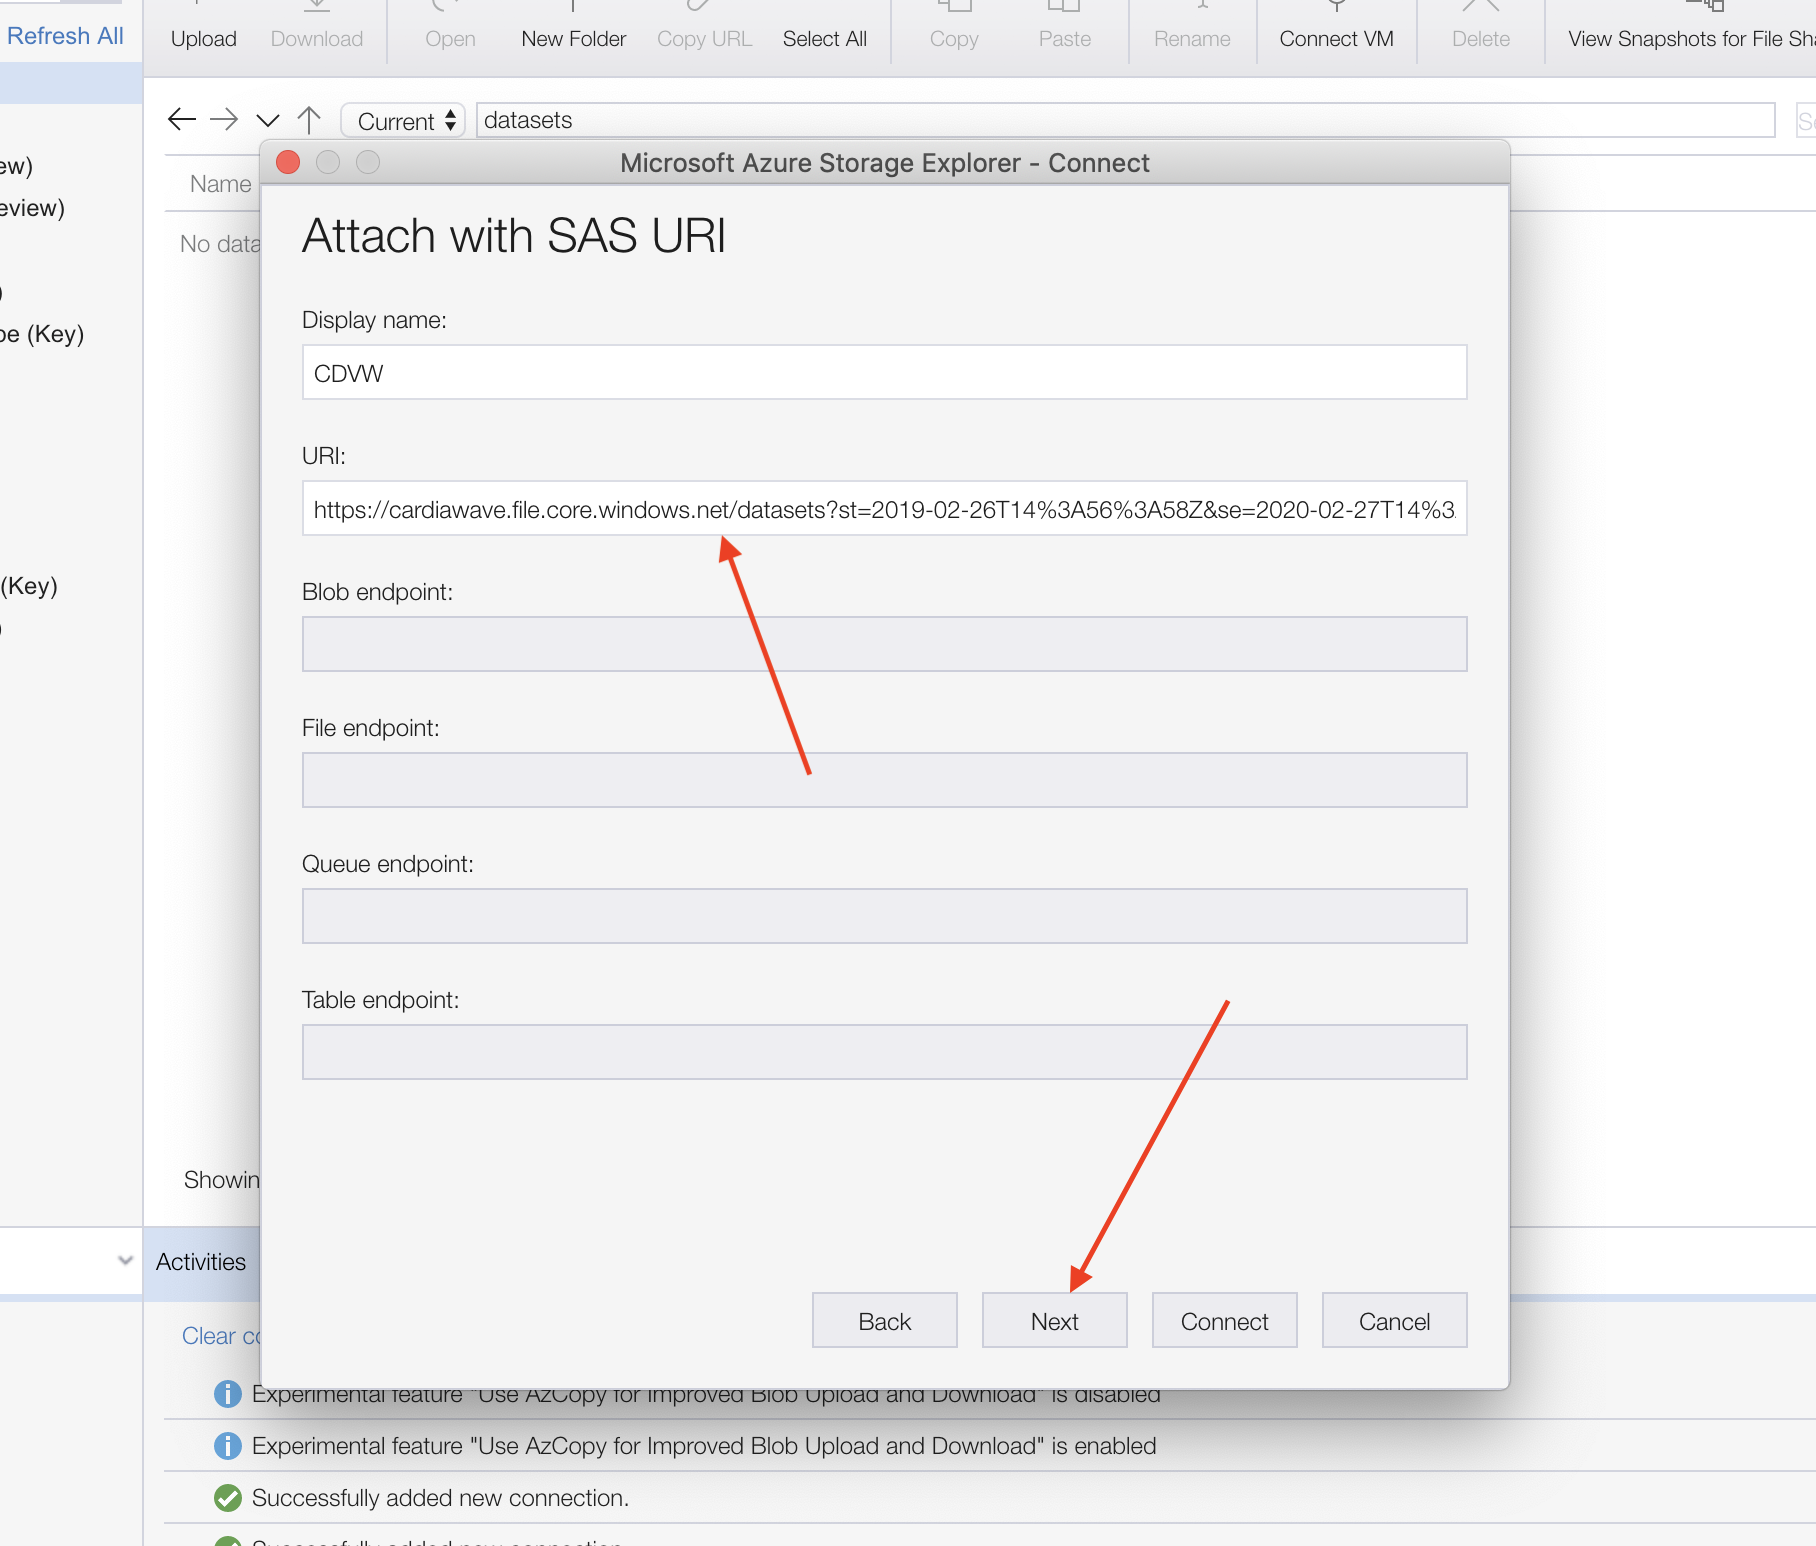
\includegraphics[width=\textwidth]{assets/az-step3.png}
        \caption{Connect to a new Azure file share}
        \label{figure:az-step3}
        \end{figure}
    \item Check the information, take note of the access expiration date and click \texttt{Connect} (see \ref{figure:az-step4})
        \begin{figure}
        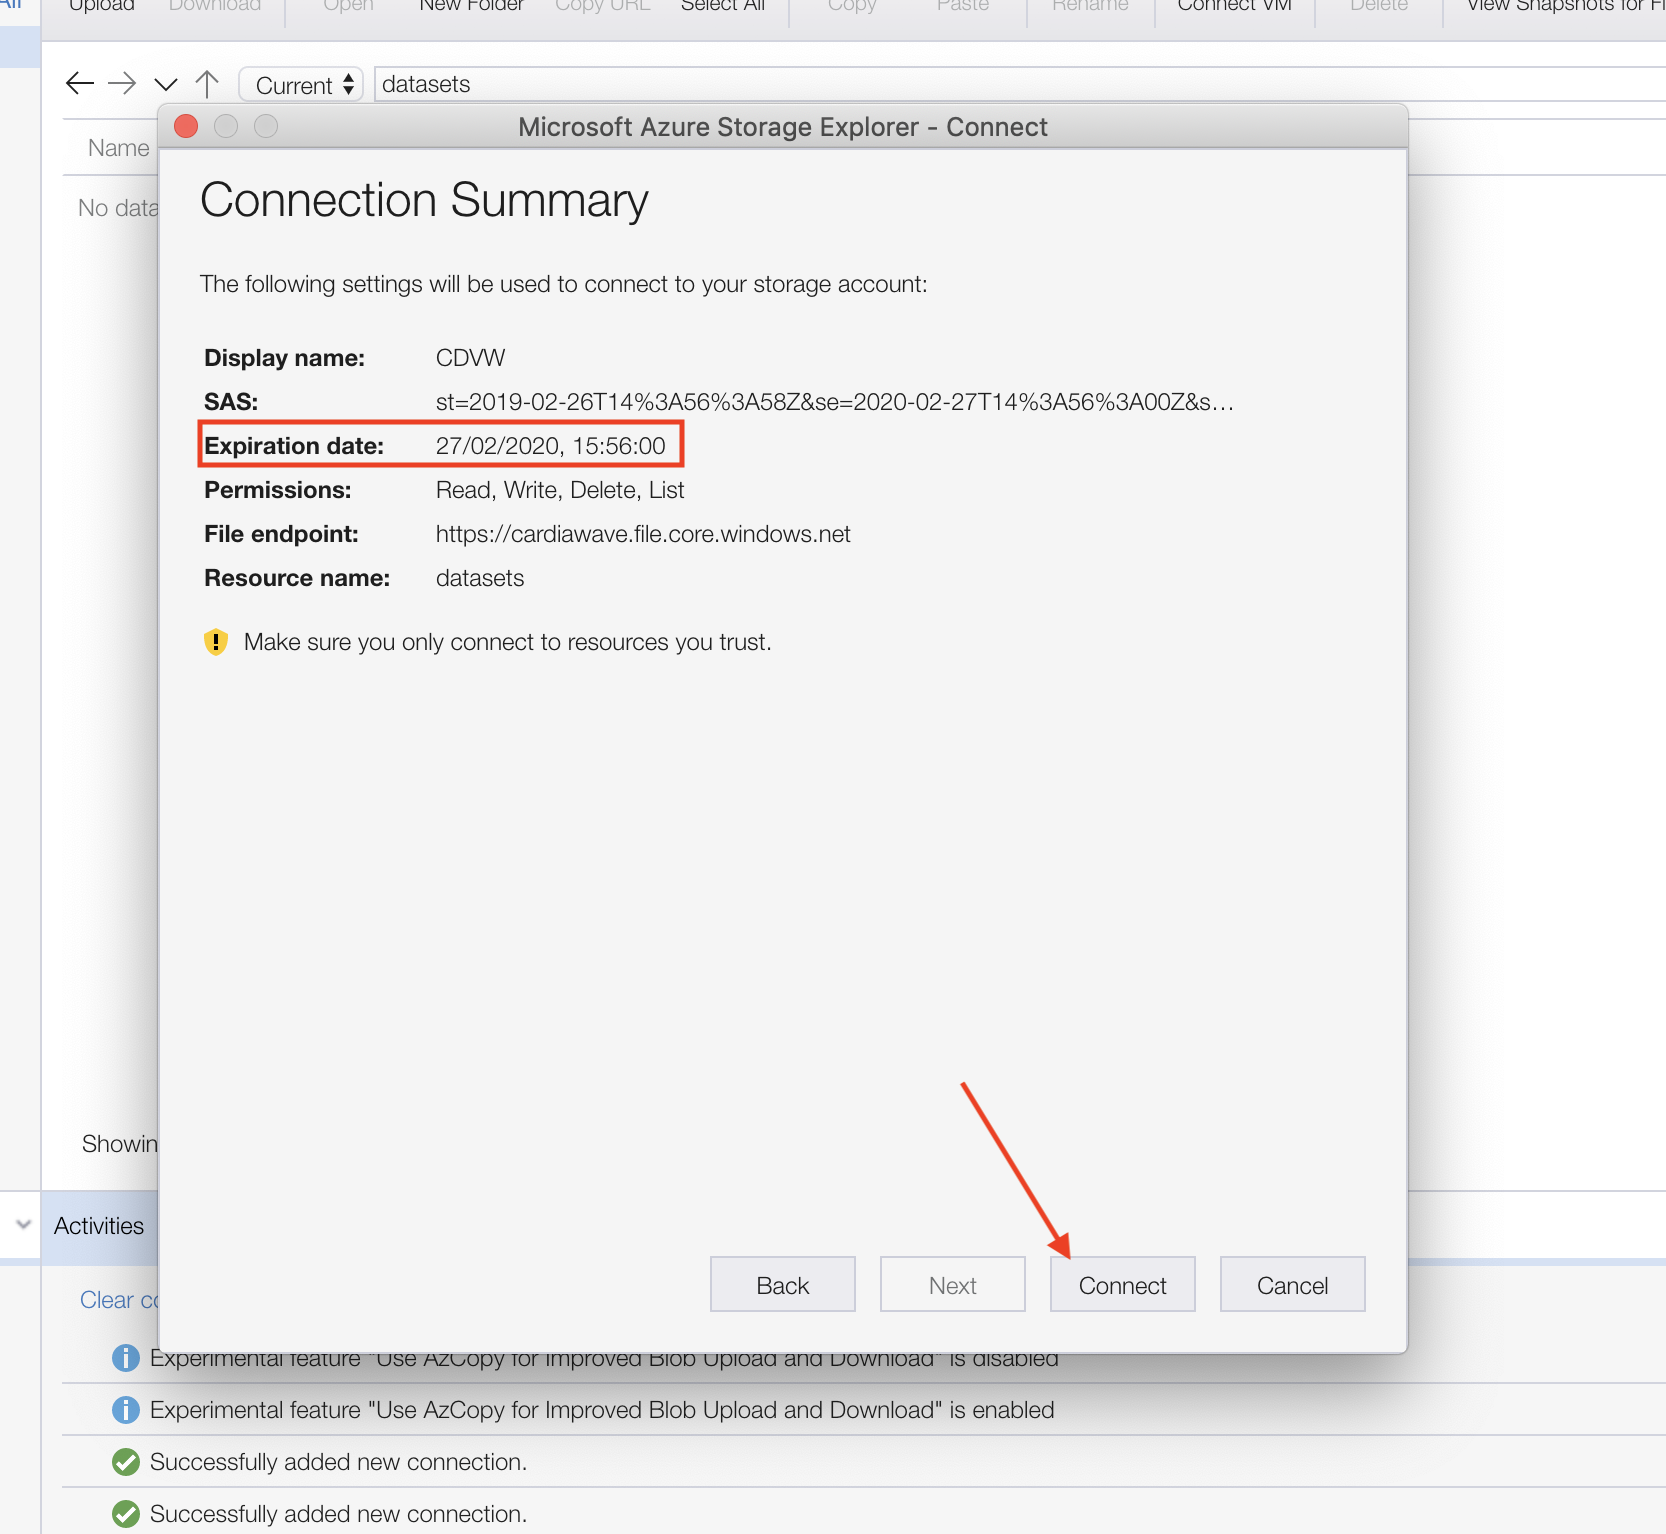
\includegraphics[width=\textwidth]{assets/az-step4.png}
        \caption{Connect to a new Azure file share}
        \label{figure:az-step4}
        \end{figure}
    \item That's it! You can use the explorer to drag and drop files to your file share, use the buttons to
    create folders, etc.
\end{itemize}
